% Options for packages loaded elsewhere
\PassOptionsToPackage{unicode}{hyperref}
\PassOptionsToPackage{hyphens}{url}
%
\documentclass[
]{article}
\usepackage{amsmath,amssymb}
\usepackage{iftex}
\ifPDFTeX
  \usepackage[T1]{fontenc}
  \usepackage[utf8]{inputenc}
  \usepackage{textcomp} % provide euro and other symbols
\else % if luatex or xetex
  \usepackage{unicode-math} % this also loads fontspec
  \defaultfontfeatures{Scale=MatchLowercase}
  \defaultfontfeatures[\rmfamily]{Ligatures=TeX,Scale=1}
\fi
\usepackage{lmodern}
\ifPDFTeX\else
  % xetex/luatex font selection
\fi
% Use upquote if available, for straight quotes in verbatim environments
\IfFileExists{upquote.sty}{\usepackage{upquote}}{}
\IfFileExists{microtype.sty}{% use microtype if available
  \usepackage[]{microtype}
  \UseMicrotypeSet[protrusion]{basicmath} % disable protrusion for tt fonts
}{}
\makeatletter
\@ifundefined{KOMAClassName}{% if non-KOMA class
  \IfFileExists{parskip.sty}{%
    \usepackage{parskip}
  }{% else
    \setlength{\parindent}{0pt}
    \setlength{\parskip}{6pt plus 2pt minus 1pt}}
}{% if KOMA class
  \KOMAoptions{parskip=half}}
\makeatother
\usepackage{xcolor}
\usepackage[margin=1.5in]{geometry}
\usepackage{color}
\usepackage{fancyvrb}
\newcommand{\VerbBar}{|}
\newcommand{\VERB}{\Verb[commandchars=\\\{\}]}
\DefineVerbatimEnvironment{Highlighting}{Verbatim}{commandchars=\\\{\}}
% Add ',fontsize=\small' for more characters per line
\usepackage{framed}
\definecolor{shadecolor}{RGB}{248,248,248}
\newenvironment{Shaded}{\begin{snugshade}}{\end{snugshade}}
\newcommand{\AlertTok}[1]{\textcolor[rgb]{0.94,0.16,0.16}{#1}}
\newcommand{\AnnotationTok}[1]{\textcolor[rgb]{0.56,0.35,0.01}{\textbf{\textit{#1}}}}
\newcommand{\AttributeTok}[1]{\textcolor[rgb]{0.13,0.29,0.53}{#1}}
\newcommand{\BaseNTok}[1]{\textcolor[rgb]{0.00,0.00,0.81}{#1}}
\newcommand{\BuiltInTok}[1]{#1}
\newcommand{\CharTok}[1]{\textcolor[rgb]{0.31,0.60,0.02}{#1}}
\newcommand{\CommentTok}[1]{\textcolor[rgb]{0.56,0.35,0.01}{\textit{#1}}}
\newcommand{\CommentVarTok}[1]{\textcolor[rgb]{0.56,0.35,0.01}{\textbf{\textit{#1}}}}
\newcommand{\ConstantTok}[1]{\textcolor[rgb]{0.56,0.35,0.01}{#1}}
\newcommand{\ControlFlowTok}[1]{\textcolor[rgb]{0.13,0.29,0.53}{\textbf{#1}}}
\newcommand{\DataTypeTok}[1]{\textcolor[rgb]{0.13,0.29,0.53}{#1}}
\newcommand{\DecValTok}[1]{\textcolor[rgb]{0.00,0.00,0.81}{#1}}
\newcommand{\DocumentationTok}[1]{\textcolor[rgb]{0.56,0.35,0.01}{\textbf{\textit{#1}}}}
\newcommand{\ErrorTok}[1]{\textcolor[rgb]{0.64,0.00,0.00}{\textbf{#1}}}
\newcommand{\ExtensionTok}[1]{#1}
\newcommand{\FloatTok}[1]{\textcolor[rgb]{0.00,0.00,0.81}{#1}}
\newcommand{\FunctionTok}[1]{\textcolor[rgb]{0.13,0.29,0.53}{\textbf{#1}}}
\newcommand{\ImportTok}[1]{#1}
\newcommand{\InformationTok}[1]{\textcolor[rgb]{0.56,0.35,0.01}{\textbf{\textit{#1}}}}
\newcommand{\KeywordTok}[1]{\textcolor[rgb]{0.13,0.29,0.53}{\textbf{#1}}}
\newcommand{\NormalTok}[1]{#1}
\newcommand{\OperatorTok}[1]{\textcolor[rgb]{0.81,0.36,0.00}{\textbf{#1}}}
\newcommand{\OtherTok}[1]{\textcolor[rgb]{0.56,0.35,0.01}{#1}}
\newcommand{\PreprocessorTok}[1]{\textcolor[rgb]{0.56,0.35,0.01}{\textit{#1}}}
\newcommand{\RegionMarkerTok}[1]{#1}
\newcommand{\SpecialCharTok}[1]{\textcolor[rgb]{0.81,0.36,0.00}{\textbf{#1}}}
\newcommand{\SpecialStringTok}[1]{\textcolor[rgb]{0.31,0.60,0.02}{#1}}
\newcommand{\StringTok}[1]{\textcolor[rgb]{0.31,0.60,0.02}{#1}}
\newcommand{\VariableTok}[1]{\textcolor[rgb]{0.00,0.00,0.00}{#1}}
\newcommand{\VerbatimStringTok}[1]{\textcolor[rgb]{0.31,0.60,0.02}{#1}}
\newcommand{\WarningTok}[1]{\textcolor[rgb]{0.56,0.35,0.01}{\textbf{\textit{#1}}}}
\usepackage{longtable,booktabs,array}
\usepackage{calc} % for calculating minipage widths
% Correct order of tables after \paragraph or \subparagraph
\usepackage{etoolbox}
\makeatletter
\patchcmd\longtable{\par}{\if@noskipsec\mbox{}\fi\par}{}{}
\makeatother
% Allow footnotes in longtable head/foot
\IfFileExists{footnotehyper.sty}{\usepackage{footnotehyper}}{\usepackage{footnote}}
\makesavenoteenv{longtable}
\usepackage{graphicx}
\makeatletter
\def\maxwidth{\ifdim\Gin@nat@width>\linewidth\linewidth\else\Gin@nat@width\fi}
\def\maxheight{\ifdim\Gin@nat@height>\textheight\textheight\else\Gin@nat@height\fi}
\makeatother
% Scale images if necessary, so that they will not overflow the page
% margins by default, and it is still possible to overwrite the defaults
% using explicit options in \includegraphics[width, height, ...]{}
\setkeys{Gin}{width=\maxwidth,height=\maxheight,keepaspectratio}
% Set default figure placement to htbp
\makeatletter
\def\fps@figure{htbp}
\makeatother
\setlength{\emergencystretch}{3em} % prevent overfull lines
\providecommand{\tightlist}{%
  \setlength{\itemsep}{0pt}\setlength{\parskip}{0pt}}
\setcounter{secnumdepth}{5}
\newlength{\cslhangindent}
\setlength{\cslhangindent}{1.5em}
\newlength{\csllabelwidth}
\setlength{\csllabelwidth}{3em}
\newlength{\cslentryspacingunit} % times entry-spacing
\setlength{\cslentryspacingunit}{\parskip}
\newenvironment{CSLReferences}[2] % #1 hanging-ident, #2 entry spacing
 {% don't indent paragraphs
  \setlength{\parindent}{0pt}
  % turn on hanging indent if param 1 is 1
  \ifodd #1
  \let\oldpar\par
  \def\par{\hangindent=\cslhangindent\oldpar}
  \fi
  % set entry spacing
  \setlength{\parskip}{#2\cslentryspacingunit}
 }%
 {}
\usepackage{calc}
\newcommand{\CSLBlock}[1]{#1\hfill\break}
\newcommand{\CSLLeftMargin}[1]{\parbox[t]{\csllabelwidth}{#1}}
\newcommand{\CSLRightInline}[1]{\parbox[t]{\linewidth - \csllabelwidth}{#1}\break}
\newcommand{\CSLIndent}[1]{\hspace{\cslhangindent}#1}
\ifLuaTeX
\usepackage[bidi=basic]{babel}
\else
\usepackage[bidi=default]{babel}
\fi
\babelprovide[main,import]{english}
% get rid of language-specific shorthands (see #6817):
\let\LanguageShortHands\languageshorthands
\def\languageshorthands#1{}
\usepackage{booktabs}
\usepackage{longtable}
\usepackage{array}
\usepackage{multirow}
\usepackage{wrapfig}
\usepackage{float}
\usepackage{colortbl}
\usepackage{pdflscape}
\usepackage{tabu}
\usepackage{threeparttable}
\usepackage{threeparttablex}
\usepackage[normalem]{ulem}
\usepackage{makecell}
\usepackage{xcolor}
\ifLuaTeX
  \usepackage{selnolig}  % disable illegal ligatures
\fi
\IfFileExists{bookmark.sty}{\usepackage{bookmark}}{\usepackage{hyperref}}
\IfFileExists{xurl.sty}{\usepackage{xurl}}{} % add URL line breaks if available
\urlstyle{same}
\hypersetup{
  pdftitle={Air Quality},
  pdfauthor={Libera Mastromatteo},
  pdflang={en},
  hidelinks,
  pdfcreator={LaTeX via pandoc}}

\title{Air Quality}
\usepackage{etoolbox}
\makeatletter
\providecommand{\subtitle}[1]{% add subtitle to \maketitle
  \apptocmd{\@title}{\par {\large #1 \par}}{}{}
}
\makeatother
\subtitle{New York Air Quality Measurement}
\author{Libera Mastromatteo}
\date{University of Padova}

\begin{document}
\maketitle

{
\setcounter{tocdepth}{4}
\tableofcontents
}
\newpage

\hypertarget{working-with-data-in-r}{%
\section{Working with Data in R}\label{working-with-data-in-r}}

\hypertarget{airquality-dataset}{%
\subsection{Airquality dataset}\label{airquality-dataset}}

The \color{red}{airquality} \normalcolor dataset is \emph{built-in} R so there is nothing to install or prepare, it is already there as an \color{green}{R} \normalcolor object. This \color{red}{data} \normalcolor  is small compared to environmental data sets.

\hypertarget{details-of-the-airquality-dataset}{%
\subsubsection{Details of the airquality dataset}\label{details-of-the-airquality-dataset}}

Daily readings of the following air quality values for May 1, 1973 a Tuesday to September 30, 1973.

\hypertarget{exploring-airquality1}{%
\paragraph[Exploring airquality]{\texorpdfstring{Exploring airquality\footnote{prova nota}}{Exploring airquality}}\label{exploring-airquality1}}

We can look at the first and last few lines of that \color{blue}{airquality} \normalcolor tabular data\footnote{questa è la mia seconda nota, c'è anche un link \color{blue}\href{https://stat.ethz.ch/R-manual/R-devel/library/datasets/html/airquality.html}{qui}\normalcolor}.

\hypertarget{proviamo-a-mettere-link}{%
\section{Proviamo a mettere link:}\label{proviamo-a-mettere-link}}

Link \href{https://www.google.com}{\textbf{qui}}

\hypertarget{vai-con-le-liste}{%
\subsection{Vai con le liste:}\label{vai-con-le-liste}}

\begin{itemize}
\tightlist
\item
  Oggi
\item
  ho
\item
  imparato
\item
  cose
\end{itemize}

\begin{enumerate}
\def\labelenumi{\arabic{enumi}.}
\tightlist
\item
  Devo
\item
  Fare
\item
  Cose
\end{enumerate}

\begin{quote}
\begin{enumerate}
\def\labelenumi{\arabic{enumi}.}
\tightlist
\item
  Devo
\item
  Fare
\item
  Cose
\end{enumerate}
\end{quote}

\hypertarget{inseriamo-delle-immagini}{%
\section{Inseriamo delle immagini}\label{inseriamo-delle-immagini}}

\begin{figure}
\centering

\includegraphics{pics/explaining-how-bad-8943e8c056.jpg}
\caption{Using Markdown code}
\end{figure}

\begin{figure}

{\centering 
\includegraphics[width=0.75\linewidth]{pics/explaining-how-bad-8943e8c056} 

}

\caption{Using RMarkdown code}\label{fig:unnamed-chunk-1}
\end{figure}
\newpage

\hypertarget{inseriamo-la-bibliografia}{%
\section{Inseriamo la bibliografia}\label{inseriamo-la-bibliografia}}

Hess and Blairy (2001) riportano che l'inquinamento fa male

Secondo recenti studi (Hess and Blairy 2001), l'inquinamento fa male

\newpage

\hypertarget{inseriamo-delle-equazioni}{%
\section{Inseriamo delle equazioni}\label{inseriamo-delle-equazioni}}

Ecco qui una bellissima equazione \(3 + 5 = 8\)

\[3 + 9 = 12\]
\[ Y = mx + q\]
\[ \Delta = 1 - \pi\]
\(\sqrt{4} = 2\)

\newpage

\hypertarget{come-inserire-cross-referencing}{%
\section{Come inserire cross-referencing}\label{come-inserire-cross-referencing}}

Come si vede in Tabella \ref{tab:cars-table1}

\begin{table}[H]

\caption{\label{tab:cars-table1}Questo è un dataset con le prime 10 righe}
\centering
\begin{tabular}[t]{l|c|c|c|c|c|c|c|c|c|c|c}
\hline
  & mpg & cyl & disp & hp & drat & wt & qsec & vs & am & gear & carb\\
\hline
Mazda RX4 & 21.0 & 6 & 160.0 & 110 & 3.90 & 2.620 & 16.46 & 0 & 1 & 4 & 4\\
\hline
Mazda RX4 Wag & 21.0 & 6 & 160.0 & 110 & 3.90 & 2.875 & 17.02 & 0 & 1 & 4 & 4\\
\hline
Datsun 710 & 22.8 & 4 & 108.0 & 93 & 3.85 & 2.320 & 18.61 & 1 & 1 & 4 & 1\\
\hline
Hornet 4 Drive & 21.4 & 6 & 258.0 & 110 & 3.08 & 3.215 & 19.44 & 1 & 0 & 3 & 1\\
\hline
Hornet Sportabout & 18.7 & 8 & 360.0 & 175 & 3.15 & 3.440 & 17.02 & 0 & 0 & 3 & 2\\
\hline
Valiant & 18.1 & 6 & 225.0 & 105 & 2.76 & 3.460 & 20.22 & 1 & 0 & 3 & 1\\
\hline
Duster 360 & 14.3 & 8 & 360.0 & 245 & 3.21 & 3.570 & 15.84 & 0 & 0 & 3 & 4\\
\hline
Merc 240D & 24.4 & 4 & 146.7 & 62 & 3.69 & 3.190 & 20.00 & 1 & 0 & 4 & 2\\
\hline
Merc 230 & 22.8 & 4 & 140.8 & 95 & 3.92 & 3.150 & 22.90 & 1 & 0 & 4 & 2\\
\hline
Merc 280 & 19.2 & 6 & 167.6 & 123 & 3.92 & 3.440 & 18.30 & 1 & 0 & 4 & 4\\
\hline
\end{tabular}
\end{table}

Come si vede in Tabella \ref{tab:cars-table}

\begin{table}[H]

\caption{\label{tab:cars-table}Questo è un dataset con le prime 5 righe}
\centering
\begin{tabular}[t]{l|r|r|r|r|r|r|r|r|r|r|r}
\hline
  & mpg & cyl & disp & hp & drat & wt & qsec & vs & am & gear & carb\\
\hline
Mazda RX4 & 21.0 & 6 & 160 & 110 & 3.90 & 2.620 & 16.46 & 0 & 1 & 4 & 4\\
\hline
Mazda RX4 Wag & 21.0 & 6 & 160 & 110 & 3.90 & 2.875 & 17.02 & 0 & 1 & 4 & 4\\
\hline
Datsun 710 & 22.8 & 4 & 108 & 93 & 3.85 & 2.320 & 18.61 & 1 & 1 & 4 & 1\\
\hline
Hornet 4 Drive & 21.4 & 6 & 258 & 110 & 3.08 & 3.215 & 19.44 & 1 & 0 & 3 & 1\\
\hline
Hornet Sportabout & 18.7 & 8 & 360 & 175 & 3.15 & 3.440 & 17.02 & 0 & 0 & 3 & 2\\
\hline
\end{tabular}
\end{table}

\hypertarget{inserire-cross-referencing-per-le-equazioni-richiede-scrittura-in-latex}{%
\subsection{Inserire cross-referencing per le equazioni richiede scrittura in LateX}\label{inserire-cross-referencing-per-le-equazioni-richiede-scrittura-in-latex}}

\begin{equation}
\bar{X} = \frac{\sum_{i=1}^n X_i}{n} \label{eq:media}
\end{equation}

Come si evince in \eqref{eq:media}

\newpage

\hypertarget{nuovo-chunck}{%
\section{Nuovo chunck}\label{nuovo-chunck}}

\begin{verbatim}
    Ozone Solar.R Wind Temp Month Day
  1    41     190  7.4   67     5   1
  2    36     118  8.0   72     5   2
  3    12     149 12.6   74     5   3
  4    18     313 11.5   62     5   4
  5    NA      NA 14.3   56     5   5
....
\end{verbatim}

\begin{center}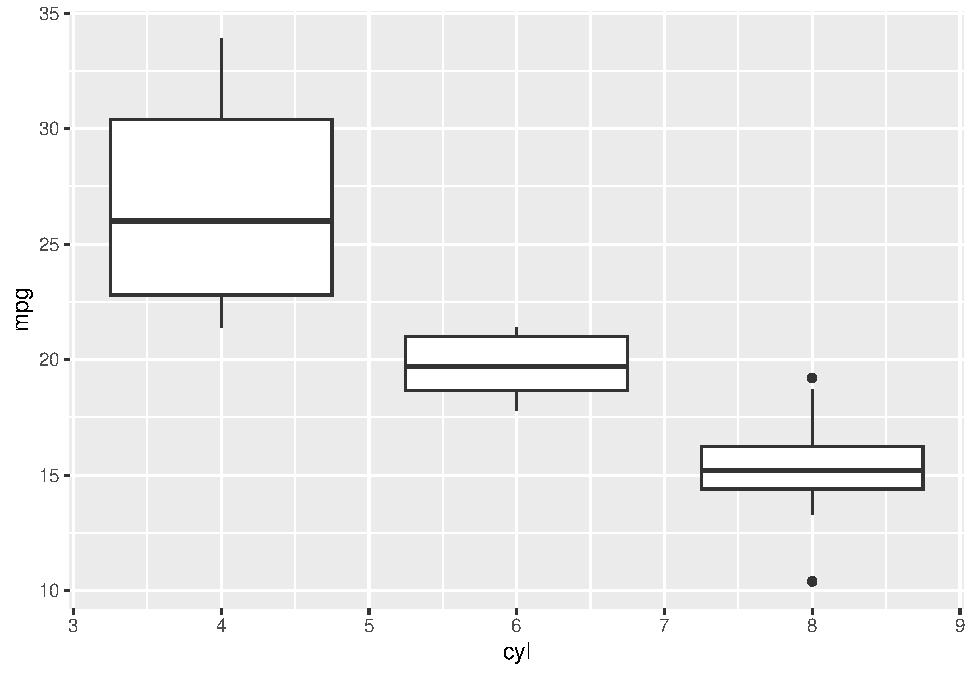
\includegraphics[width=0.5\linewidth]{Airquality2_files/figure-latex/unnamed-chunk-3-1} \end{center}

\hypertarget{esercitazione}{%
\section{Esercitazione}\label{esercitazione}}

\hypertarget{summary}{%
\subsection{Summary}\label{summary}}

\begin{verbatim}
NA      Ozone           Solar.R           Wind             Temp      
NA  Min.   :  1.00   Min.   :  7.0   Min.   : 1.700   Min.   :56.00  
NA  1st Qu.: 18.00   1st Qu.:115.8   1st Qu.: 7.400   1st Qu.:72.00  
NA  Median : 31.50   Median :205.0   Median : 9.700   Median :79.00  
NA  Mean   : 42.13   Mean   :185.9   Mean   : 9.958   Mean   :77.88  
NA  3rd Qu.: 63.25   3rd Qu.:258.8   3rd Qu.:11.500   3rd Qu.:85.00  
NA  Max.   :168.00   Max.   :334.0   Max.   :20.700   Max.   :97.00  
NA  NA's   :37       NA's   :7                                       
NA      Month            Day      
NA  Min.   :5.000   Min.   : 1.0  
NA  1st Qu.:6.000   1st Qu.: 8.0  
NA  Median :7.000   Median :16.0  
NA  Mean   :6.993   Mean   :15.8  
NA  3rd Qu.:8.000   3rd Qu.:23.0  
NA  Max.   :9.000   Max.   :31.0  
NA 
\end{verbatim}

\hypertarget{plot-1}{%
\subsection{Plot 1}\label{plot-1}}

\begin{center}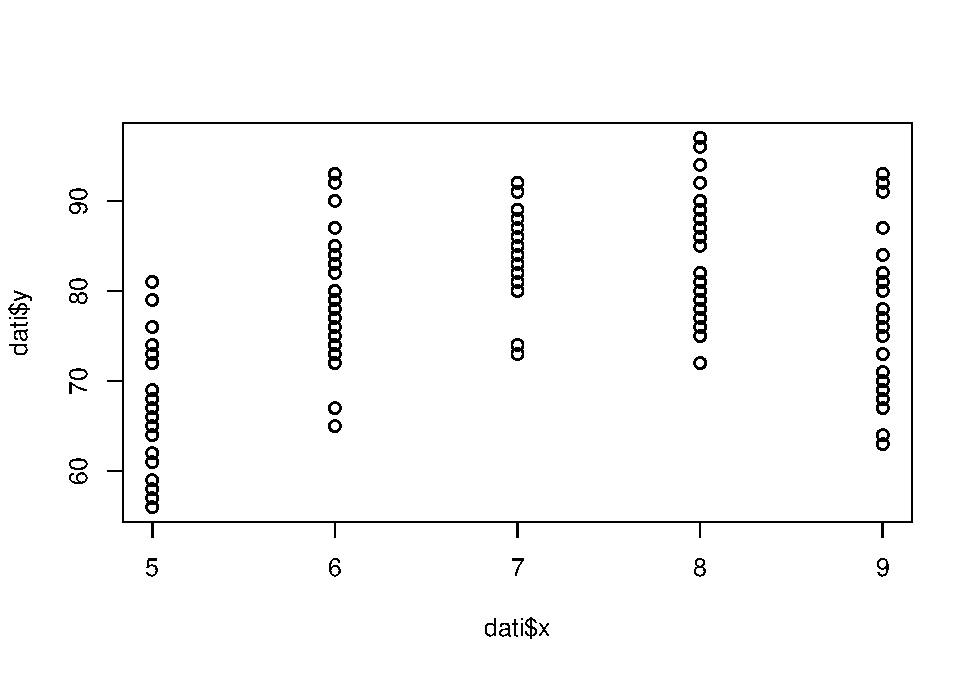
\includegraphics[width=0.5\linewidth]{Airquality2_files/figure-latex/unnamed-chunk-6-1} \end{center}

\hypertarget{plot-2}{%
\subsection{Plot 2}\label{plot-2}}

\begin{Shaded}
\begin{Highlighting}[]
\FunctionTok{plot}\NormalTok{(dati}\SpecialCharTok{$}\NormalTok{y }\SpecialCharTok{\textasciitilde{}}\NormalTok{ dati}\SpecialCharTok{$}\NormalTok{x)}
\end{Highlighting}
\end{Shaded}

\hypertarget{first-10-rows}{%
\subsection{First 10 rows}\label{first-10-rows}}

\begin{verbatim}
NA    Ozone Solar.R Wind Temp Month Day  y x
NA 1     41     190  7.4   67     5   1 67 5
NA 2     36     118  8.0   72     5   2 72 5
NA 3     12     149 12.6   74     5   3 74 5
NA 4     18     313 11.5   62     5   4 62 5
NA 5     NA      NA 14.3   56     5   5 56 5
NA 6     28      NA 14.9   66     5   6 66 5
NA 7     23     299  8.6   65     5   7 65 5
NA 8     19      99 13.8   59     5   8 59 5
NA 9      8      19 20.1   61     5   9 61 5
NA 10    NA     194  8.6   69     5  10 69 5
....
\end{verbatim}

\hypertarget{tabelle}{%
\section{Tabelle}\label{tabelle}}

\begin{longtable}[]{@{}llllll@{}}
\toprule\noalign{}
X & Y & Z & W & A & U \\
\midrule\noalign{}
\endhead
\bottomrule\noalign{}
\endlastfoot
1 & 1 & 1 & NA & C & \\
B & B & B & S & 0 & \\
NA & 2 & 3 & 3 & 3 & \\
\end{longtable}

\begin{longtable}[]{@{}lcrl@{}}
\toprule\noalign{}
Tables & Are & Cool & new column \\
\midrule\noalign{}
\endhead
\bottomrule\noalign{}
\endlastfoot
col 1 is & left-aligned & \$1600 & . \\
col 2 is & centered & \$12 & . \\
col 3 is & right-aligned & \$1 & . \\
\end{longtable}

\begin{longtable}[]{@{}rlc@{}}
\toprule\noalign{}
Tables & Are & Cool \\
\midrule\noalign{}
\endhead
\bottomrule\noalign{}
\endlastfoot
1 is & right-aligned & \$1600 \\
2 is & left-aligned & \$12 \\
3 is & centered & \$1 \\
\end{longtable}

\hypertarget{tabelle-con-codice-r}{%
\subsection{Tabelle con codice R}\label{tabelle-con-codice-r}}

\begin{verbatim}
## 
## Please cite as:
\end{verbatim}

\begin{verbatim}
##  Hlavac, Marek (2022). stargazer: Well-Formatted Regression and Summary Statistics Tables.
\end{verbatim}

\begin{verbatim}
##  R package version 5.2.3. https://CRAN.R-project.org/package=stargazer
\end{verbatim}

\begin{table}[!htbp] \centering 
  \caption{Tabella di summary} 
  \label{} 
\begin{tabular}{@{\extracolsep{5pt}}lccccc} 
\\[-1.8ex]\hline 
\hline \\[-1.8ex] 
Statistic & \multicolumn{1}{c}{N} & \multicolumn{1}{c}{Mean} & \multicolumn{1}{c}{St. Dev.} & \multicolumn{1}{c}{Min} & \multicolumn{1}{c}{Max} \\ 
\hline \\[-1.8ex] 
Ozone & 116 & 42.129 & 32.988 & 1 & 168 \\ 
Solar.R & 146 & 185.932 & 90.058 & 7 & 334 \\ 
Wind & 153 & 9.958 & 3.523 & 1.700 & 20.700 \\ 
Temp & 153 & 77.882 & 9.465 & 56 & 97 \\ 
Month & 153 & 6.993 & 1.417 & 5 & 9 \\ 
Day & 153 & 15.804 & 8.865 & 1 & 31 \\ 
y & 153 & 77.882 & 9.465 & 56 & 97 \\ 
x & 153 & 6.993 & 1.417 & 5 & 9 \\ 
\hline \\[-1.8ex] 
\end{tabular} 
\end{table}

\begin{table}[!htbp] \centering 
  \caption{Risultati del modello} 
  \label{} 
\begin{tabular}{@{\extracolsep{5pt}}lc} 
\\[-1.8ex]\hline 
\hline \\[-1.8ex] 
 & \multicolumn{1}{c}{\textit{Dependent variable:}} \\ 
\cline{2-2} 
\\[-1.8ex] & Temp \\ 
\hline \\[-1.8ex] 
 Constant & 58.211$^{***}$ \\ 
  & (3.519) \\ 
  & \\ 
 Month & 2.813$^{***}$ \\ 
  & (0.493) \\ 
  & \\ 
\hline \\[-1.8ex] 
Observations & 153 \\ 
R$^{2}$ & 0.177 \\ 
Adjusted R$^{2}$ & 0.172 \\ 
Residual Std. Error & 8.614 (df = 151) \\ 
F Statistic & 32.519$^{***}$ (df = 1; 151) \\ 
\hline 
\hline \\[-1.8ex] 
\textit{Note:}  & \multicolumn{1}{r}{$^{*}$p$<$0.1; $^{**}$p$<$0.05; $^{***}$p$<$0.01} \\ 
\end{tabular} 
\end{table}

\begin{table}[H] \centering 
  \caption{Risultati del modello} 
  \label{tab:model.comparison} 
\begin{tabular}{@{\extracolsep{5pt}}lcc} 
\\[-1.8ex]\hline 
\hline \\[-1.8ex] 
 & \multicolumn{2}{c}{\textit{Dependent variable:}} \\ 
\cline{2-3} 
\\[-1.8ex] & \multicolumn{2}{c}{Temp} \\ 
\\[-1.8ex] & (1) & (2)\\ 
\hline \\[-1.8ex] 
 Constant & 77.882$^{***}$ & 58.211$^{***}$ \\ 
  & (0.765) & (3.519) \\ 
  & & \\ 
 Month &  & 2.813$^{***}$ \\ 
  &  & (0.493) \\ 
  & & \\ 
\hline \\[-1.8ex] 
Observations & 153 & 153 \\ 
R$^{2}$ & 0.000 & 0.177 \\ 
Adjusted R$^{2}$ & 0.000 & 0.172 \\ 
Residual Std. Error & 9.465 (df = 152) & 8.614 (df = 151) \\ 
F Statistic &  & 32.519$^{***}$ (df = 1; 151) \\ 
\hline 
\hline \\[-1.8ex] 
\textit{Note:}  & \multicolumn{2}{r}{$^{*}$p$<$0.1; $^{**}$p$<$0.05; $^{***}$p$<$0.01} \\ 
\end{tabular} 
\end{table}

Come si vede in Tabella \ref{tab:model.comparison}, qui c'è un confronto tra \(m0\) e \(m1\).

\[x = \frac{-10.8823529}{9.4652697} =-1.149714\]

\[x = \frac{-10.8823529}{9.4652697} =-1.149714\]

\begin{center}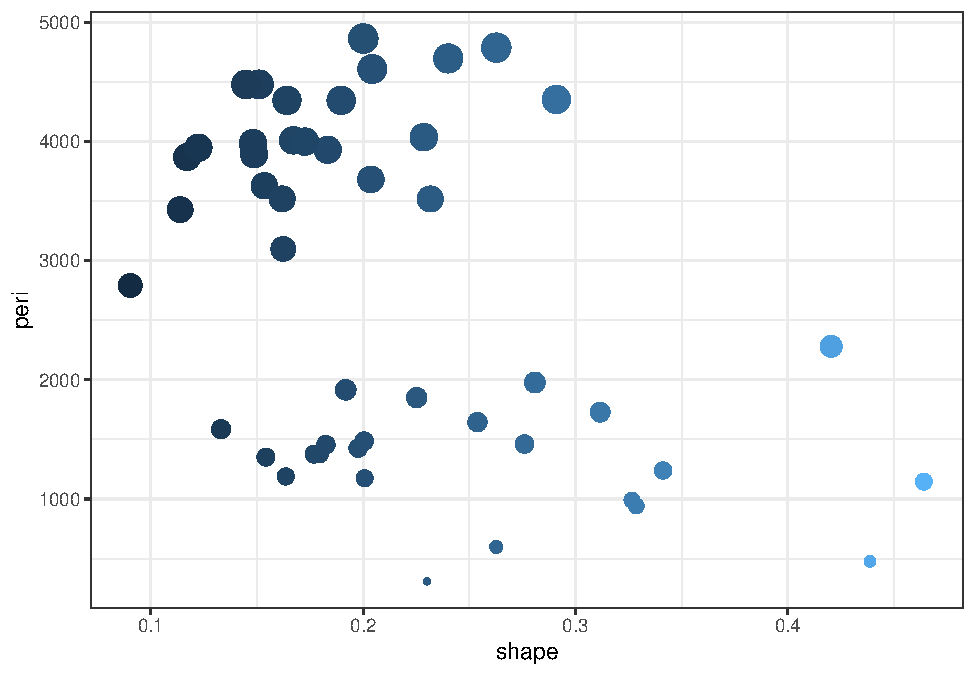
\includegraphics[width=0.5\linewidth]{Airquality2_files/figure-latex/plot-static-1} \end{center}

\color{red} Voglio una frase rossa \normalcolor

\newpage

\hypertarget{references}{%
\section*{References}\label{references}}
\addcontentsline{toc}{section}{References}

\hypertarget{refs}{}
\begin{CSLReferences}{1}{0}
\leavevmode\vadjust pre{\hypertarget{ref-hess2001facial}{}}%
Hess, Ursula, and Sylvie Blairy. 2001. {``Facial Mimicry and Emotional Contagion to Dynamic Emotional Facial Expressions and Their Influence on Decoding Accuracy.''} \emph{International Journal of Psychophysiology} 40 (2): 129--41.

\end{CSLReferences}

\end{document}
